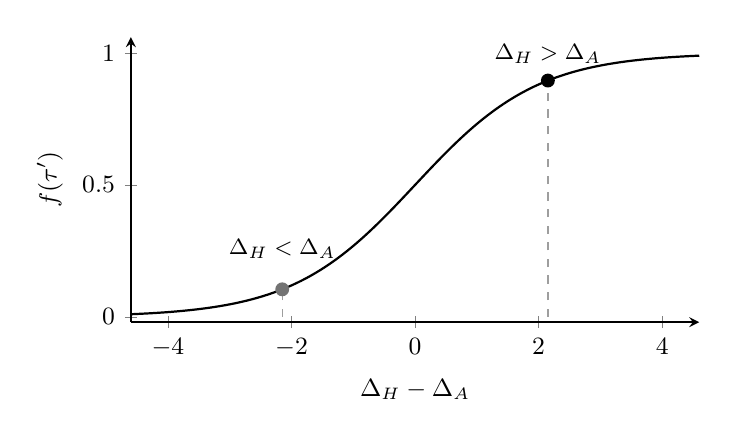
\begin{tikzpicture}
\begin{axis}[
  width=8.8cm,
  height=5.2cm,
  xmin=-4.6,
  xmax=4.6,
  ymin=-0.02,
  ymax=1.06,
  axis lines=left,
  xlabel={$\Delta_H - \Delta_A$},
  xlabel style={yshift=-1.5pt},
  ylabel={$f(\tau')$},
  xtick={-4,-2,0,2,4},
  ytick={0,0.5,1},
  tick label style={font=\small},
  label style={font=\small},
  line width=0.6pt,
  clip=false,
  enlarge x limits=false,
]
\addplot[
  thick,
  domain=-4.6:4.6,
  samples=201,
  smooth,
] {1/(1+exp(-x))};
\draw[dashed, line width=0.45pt, black!38]
  (axis cs:-2.15,0) -- (axis cs:-2.15,{1/(1+exp(2.15))});
\draw[dashed, line width=0.45pt, black!38]
  (axis cs:2.15,0) -- (axis cs:2.15,{1/(1+exp(-2.15))});
\addplot[only marks, mark=*, mark size=2.2pt, forget plot, draw=black!55, fill=black!55]
  coordinates {(-2.15, {1/(1+exp(2.15))})};
\addplot[only marks, mark=*, mark size=2.2pt, forget plot, draw=black, fill=black]
  coordinates {(2.15, {1/(1+exp(-2.15))})};
\node[font=\footnotesize, anchor=south, inner sep=11pt] at (axis cs:-2.15,{1/(1+exp(2.15))}) {$\Delta_H<\Delta_A$};
\node[font=\footnotesize, anchor=south, inner sep=6pt] at (axis cs:2.15,{1/(1+exp(-2.15))}) {$\Delta_H>\Delta_A$};
\end{axis}
\end{tikzpicture}
